% @author Benjamin Schröder
%
\chapter{Implementierung}
Im folgenden Kapitel betrachten wir die praktische Implementierung der zuvor vorgestellten Konzepte. Dazu werden zunächst
einige spezifische Anforderungen an die zu entwickelnde Software aufgelistet. Anschließend wird darauf eingegangen, wie
diese Anforderungen dann umgesetzt werden, indem die verwendeten Technologien und Entwurfsmuster vorgestellt werden.

\section{Anforderungen an die Software}
\subsection{Funktionale Anforderungen}
Die funktionalen Anforderungen beschreiben, \textit{was} umgesetzt werden soll, also welche konkreten Funktionen von der Software
bereitgestellt werden sollen. Diese lauten wie folgt:

\begin{itemize}
    \item es sollen beliebige polygonale 2D-Strukturen als Input eingelesen werden können
    \item es sollen einige Beispielstrukturen als Input zur Verfügung gestellt werden, zwischen denen der Nutzer auswählen kann
    \item mithilfe einer polygonalen Struktur als Input sollen automatisch ähnliche Strukturen generiert werden können:
    \begin{itemize}
        \item aus einer eingelesenen Inputstruktur sollen automatisch Regeln für eine Graphgrammatik abgeleitet werden können
        \item aus einer gegebenen Graphgrammatik sollen verschiedene Graphen abgeleitet werden können
        \item aus einem solchen Graphen soll dann eine planare Outputstruktur mit fester Geometrie (also festen Knotenpositionen) erzeugt werden können
    \end{itemize}
    \item es soll eine Benutzeroberfläche geben, in welcher der Nutzer Parameter für die Generierung einstellen sowie verschiedene Inputstrukturen auswählen können soll
    \item sowohl die Inputstrukturen, die daraus erzeugt Grammatik und die generierten Variationen sollen visualisiert werden können
\end{itemize}

\subsection{Nicht-funktionale Anforderungen}
Die nicht-funktionalen Anforderungen beschreiben, \textit{wie} die oben aufgelisteten Funktionen umgesetzt werden sollen, also
welche Qualitätskriterien dabei eingehalten werden sollen. Diese lauten wie folgt:

\begin{itemize}
    \item die Anwendung soll auf Windows ausführbar sein
    \item die Nutzeroberfläche soll einfach und übersichtlich gehalten werden
    \item die implementierten Algorithmen sollen sich deterministisch verhalten und durch einen Seed reproduzierbar sein
    \item alle wichtigen Komponenten sollen durch Tests abgedeckt sein
    \item alle nicht-trivialen Bestandteile des Codes sollen mit Kommentaren versehen werden
\end{itemize}

\section{Verwendete Technologien und Bibliotheken}
Der gesamte Code ist in Java 16 geschrieben. Die grafische Benutzeroberfläche wird mithilfe des Java GUI-Toolkits Swing umgesetzt,
welches Bestandteil der Java-Runtime ist und viele Bibliotheken zum Erstellen von simplen Nutzeroberflächen bereitstellt. Zum Rendern
der erzeugten Strukturen wird die \code{Graphics} Komponente des Abstract Window Toolkits (AWT) verwendet, welches ebenfalls ein
Teil der Java-Runtime ist. Die entwickelte Software wird hierbei als Teil eines größeren \gls{ac:pcg}-Projekts von Prof. Dr. Philipp Jenke umgesetzt,
in welchem sich viele weitere Studenten-Projekte, sowie Implementierungen von weiteren Algorithmen und Datenstrukturen im Bereich der prozeduralen
Generierung befinden. Die grundsätzlichen von uns verwendeten Datenstrukturen und Algorithmen werden jedoch allesamt selbst implementiert
und wir bedienen uns lediglich einiger Helfer-Funktionen, z.B. für das Einlesen von Dateien oder dem Loggen des Programmablaufs.

\section{Architektur}

\begin{figure}[h]
    \centering
    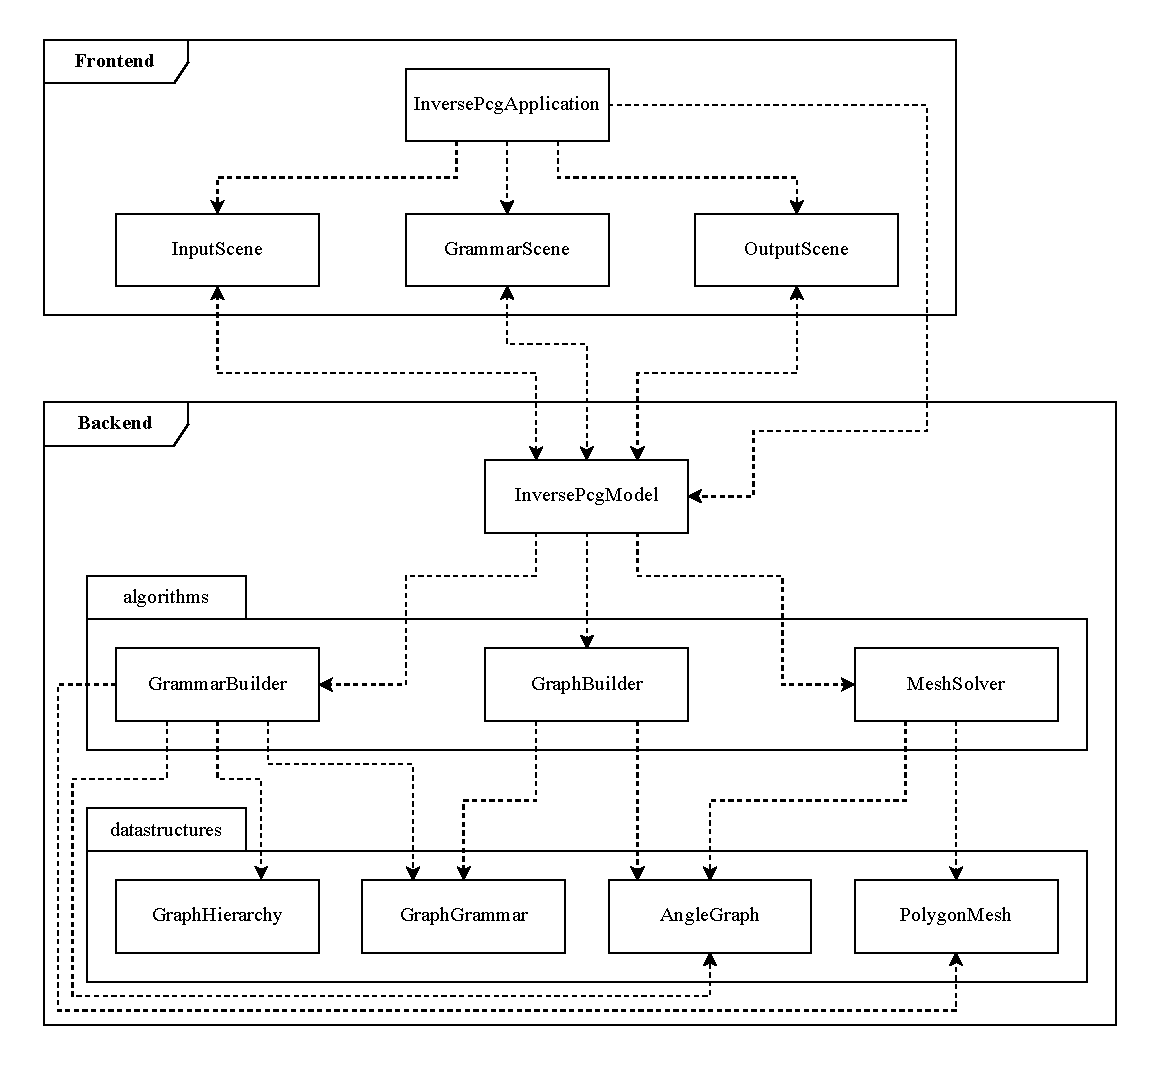
\includegraphics[width=\textwidth]{images/architecture.pdf}
    \caption{Architektur der entwickelten Software.}
    \label{fig:architecture}
\end{figure}

Um ein solches Softwareprojekt übersichtlich zu halten und in eine logische Struktur zu bringen, ist das Verwenden bestimmter Entwurfsmuster nötig.
Wie in Abbildung \ref{fig:architecture} zu sehen ist, bedienen wir uns hierfür dem bewährten Muster \textit{\gls{ac:mvc}}.

Das \gls{ac:mvc} Entwurfsmuster beschreibt drei separate logische Einheiten bzw. Komponenten. Das \textit{Datenmodell (model)} verwaltet alle für
die Anwendung wichtigen Daten und steht somit im Mittelpunkt. Das Datenmodell ist von den anderen Komponenten unabhängig und speichert die Daten einheitlich
ab. Die anderen Komponenten können beliebig ausgetauscht werden, ohne dass das Datenmodell auf diese angepasst werden muss. Die \textit{Ansicht (view)}
ist für die Darstellung der Daten des Datenmodells zuständig und realisiert die Interaktion mit dem Endnutzer durch Bereitstellen einer Benutzeroberfläche.
Die entsprechenden Daten werden von dieser Komponente nur dargestellt, nicht aber anderweitig verarbeitet. Für die Verarbeitung der Daten ist die
\textit{Steuerung (controller)} verantwortlich. Die Ansicht ist von der Steuerung unabhängig, da diese alle darzustellenden Daten ausschließlich aus
dem Datenmodell bezieht. Die Steuerung wird von der Ansicht über Anfragen des Endnutzers informiert, verarbeitet diese und aktualisiert anschließend das
Datenmodell. Die Ansicht wird daraufhin vom Datenmodell über die Änderung der Daten informiert und aktualisiert die Darstellung. \cite{48_bucanek}

In unserem Fall werden diese Komponenten wie folgt umgesetzt: Die Ansicht wird durch die Frontend-Komponenten realisiert, das Datenmodell wird in der
Klasse \code{InversePcgModel} umgesetzt und die Steuerung setzt sich zusammen aus den Klassen \code{InversePcgController}, \code{GrammarBuilder},
\code{GraphBuilder}, und \code{MeshSolver}. Im Datenmodell sind neben den zu visualisierenden Datenstrukturen ebenfalls Parameter gespeichert,
welche von der Steuerung zum Verarbeiten der Daten benutzt werden. Diese Parameter können in der Benutzeroberfläche angepasst werden, woraufhin die
Ansicht die Parameterwerte im Datenmodell direkt anpasst. Die Steuerung bietet Schnittstellen an, welche von der Ansicht genutzt werden, um
die Befehle des Benutzers auszuführen. Nach der Ausführung dieser Befehle nimmt die Steuerung Änderungen am Datenmodell vor, was von der Ansicht bemerkt
wird, da die dort enthaltenen Szenen das Beobachter-Muster (Observer-Pattern) nutzen, um auf Änderungen im Datenmodell zu lauschen. Wird das Datenmodell
geändert, so werden alle Beobachter darüber informiert. Anschließend wird die Darstellung der visualisierten Datenstrukturen in der Ansicht angepasst.

Dies sollte einen groben Überblick über den Aufbau der entwickelten Software geschafft haben. In den folgenden Kapiteln werden nun weitere Details
zur Implementierung der einzelnen Komponenten vorgestellt.

\section{Datenstrukturen}
Schauen wir uns zunächst die implementierten Datenstrukturen etwas genauer an. Diese stellen unseren Input und Output dar, werden von den implementierten
Algorithmen verarbeitet und durch die Benutzeroberfläche visualisiert. Grundsätzlich werden dabei vier verschiedene Datenstrukturen implementiert, die nun
betrachtet werden.

\subsection{PolygonMesh}
Die \code{PolygonMesh} Klasse repräsentiert die in \autoref{chap:input} vorgestellte polygonale Struktur, die der Algorithmus
als Input bekommt und als Output erzeugt. Jedes \code{PolygonMesh} Objekt verwaltet eine Liste von Knoten (Klasse \code{Vertex}),
eine Liste von Kanten (Klasse \code{Edge}) und eine Liste von Polygonen (Klasse \code{Polygon}). Diese werden alle auf der
obersten Ebene (also in der \code{PolygonMesh} Klasse) verwaltet, um das Erzeugen von Duplikaten zu verhindern. Da sich
mehrere Polygone die gleichen Kanten, und mehrere Kanten die gleichen Knoten teilen können, kann es sonst vorkommen, dass diese mehrfach
in der Datenstruktur gespeichert werden. Durch die Verwaltung aller Instanzen der anderen Klassen in \code{PolygonMesh} selbst wird
dies verhindert.

Ein \code{Vertex} besitzt lediglich nur ein einziges Feld: eine zweidimensionale Knotenposition und kann dadurch vollständig
beschrieben werden. Eine \code{Edge} wird durch zwei verschiedene Knoten definiert. Für diese wird jeweils nur ein Index gespeichert,
über welchen das eigentliche \code{Vertex} Objekt in der Knotenliste in \code{PolygonMesh} referenziert werden kann. Die Felder in
\code{Polygon} werden ähnlich umgesetzt: auch hier werden wieder nur Indexe für die untergeordneten Objekte gespeichert. Jedes
\code{Polygon} besitzt dabei eine Liste von Kanten- als auch Knoten-Indexen. Außerdem enthält jedes \code{Polygon} ein Feld
für eine Farbe, welche später genutzt wird, um dieses in der grafischen Darstellung einzufärben.

Neben der Verwaltung der eigentlichen Datenstruktur stellt die \code{PolygonMesh} Klasse außerdem Funktionalität zum Serialisieren
und Deserialisieren der Objekte bereit. Ein \code{PolygonMesh} Objekt kann in eine \code{.mesh} Datei umgewandelt werden und umgekehrt
kann ein neues \code{PolygonMesh} Objekt durch das Einlesen einer \code{.mesh} Datei initialisiert werden. So können wir neue
\code{PolygonMesh} Objekte zur Laufzeit erzeugen. In einer \code{.mesh} Datei werden alle Knotenpositionen, die Knoten-Indexe der einzelnen
Polygone, sowie die Polygonfarben als Plain-Text abgespeichert. Dies ermöglicht das einfache Erstellen von neuen Polygon-Strukturen, die
dann dem Nutzer als Input für den Algorithmus bereitgestellt werden können.

\subsection{AngleGraph}
Die \code{AngleGraph} Datenstruktur implementiert den in \autoref{chap:winkelgraph} vorgestellten Winkelgraphen. Zusätzlich zur
\code{AngleGraph} Klasse selbst, implementieren wir hier die Klassen \code{AngleEdge} und \code{AngleHalfEdge}, die die Kanten
und Halbkanten repräsentieren, als auch eine innere Klasse \code{GraphBoundary}, die den \gls{ac:gbs} des jeweiligen Graphen
darstellt. Eine eigene Klasse für die Knoten eines Winkelgraphen gibt es nicht, da diese in einem Winkelgraphen keine Eigenschaften
besitzen. Stattdessen wird in \code{AngleGraph} nur die Gesamtanzahl \(n\) aller vorhandenen Knoten gespeichert, während die Kanten
und Halbkanten statt Referenzen auf ein Knoten-Objekt lediglich Knoten-IDs von \(0\) bis \(n - 1\) zugeordnet bekommen.
Eine \code{AngleEdge} enthält zwei solcher Knoten-IDs, während die \code{AngleHalfEdge} nur an einem Knoten anliegt. Beide Kantentypen
enthalten außerdem einen Tangentenwinkel. Die \code{GraphBoundary} verwaltet eine Liste an Indexen der enhaltenen Halbkanten, sowie
Referenzen zu den sich daraus ergebenden positiven und negativen Drehungen, welche durch festgelegte Zahlenwerte repräsentiert werden.

Außerdem wird auch hier einiges an Funktionalität bereitgestellt. Der \gls{ac:gbs} kann automatisch aus den vorhandenen Halbkanten
abgeleitet werden. Es gibt einige Konstruktoren für verschiedene Anwendungsfälle, darunter einen, der ein \code{PolygonMesh} in
einen Winkelgraphen umwandeln kann. Außerdem wird ein tiefgehender Objektvergleich implementiert, welcher die zugrundeliegende Struktur
der einzelnen Winkelgraphen miteinander vergleicht. Dies erleichtert das Finden von Duplikaten beim Erstellen der
Graph-Hierarchie immens. Für die \code{GraphBoundary} wird Funktionalität bereitgestellt, die diesen in eine auf den
Kantenwinkeln basierende Darstellung umwandeln kann, welche zwischen allen Winkelgraphen einheitlich verglichen werden kann und somit
das Ableiten von Regeln für die Graphgrammatik ermöglicht.

\subsection{GraphHierarchy}
Die Graph-Hierarchie ist eine vergleichsweise simple Datenstruktur und ist vollständig in der Klasse \code{GraphHierarchy} implementiert.
Diese enthält eine Liste für die verschiedenen Generationen, welche sich jeweils aus einer Reihe an \code{AngleGraph} Objekten
zusammensetzen. Außerdem existiert ein Feld für die aktuelle Größe der Hierarchie, welche die aktuelle Anzahl an darin enthaltenen
Winkelgraphen darstellt.

\subsection{GraphGrammar}
Die finale Datenstruktur implementiert die Graphgrammatik. Diese ist ebenfalls in einer einzigen Klasse \code{GraphGrammar} implementiert.
Hier werden zwei Listen verwaltet: eine für die Starter-Regeln und eine für alle anderen Regeln. Starter-Regeln bestehen ausschließlich
aus einem \code{AngleGraph}, da die andere Seite einer solchen Regel den leeren Graphen enthält, welcher nicht explizit repräsentiert
werden muss. Alle anderen Regeln werden durch ein Paar von Winkelgraphen gebildet, welche jeweils die linke und die rechte Seite der
Regel repräsentieren.

\section{Datenmodell}
Betrachten wir nun das Datenmodell. Dieses wird in der Klasse \code{InversePcgModel} realisiert. Dieses enthält Felder für die polygonale
Inputstruktur, die daraus erzeugte Grammatik, sowie für die letztendlich erzeugte polygonale Outputstruktur. Außerdem werden hier alle
für die Steuerung relevanten Parameter verwaltet, welche zunächst im Konstruktor mit vorgebenen Standardwerten initialisiert werden und
anschließend vom Benutzer beliebig angepasst werden können. Die Liste an vorhandenen Parametern lautet wie folgt:

\begin{itemize}
    \item \code{seed}: der Seed für die von den Algorithmen verwendeten Zufallsgeneratoren
    \item \code{maxGeneration}: die Maximalanzahl an Generationen in der Graph-Hierarchie beim Erstellen der Graphgrammatik
    \item \code{iterations}: die Anzahl an Iterationen beim Ableiten von neuen Winkelgraphen aus der Graphgrammatik
    \item \code{maxTries}: die maximale Anzahl an Versuchen für das Erzeugen einer validen Zeichnung für einen erzeugten Graphen
    \item \code{minRandVal}: der kleinstmögliche Zufallswert für die freien Variablen beim Erzeugen einer Graph-Zeichnung
    \item \code{maxRandVal}: der größtmögliche Zufallswert für die freien Variablen beim Erzeugen einer Graph-Zeichnung
    \item \code{waitTime}: die Wartezeit zwischen den einzelnen Iterationen beim Erzeugen des Outputs
\end{itemize}

Zum Umsetzen des Beobachter-Musters erweitert \code{InversePcgModel} die Klasse \code{Observable}, welche erneut von Prof. Dr. Philipp Jenke
bereitgestellt wird. Diese erlaubt das Hinzufügen von \code{Observer} Objekten, die dann durch die ebenfalls gegebene Methode
\code{notifyAllObservers} über Änderungen am Datenmodell informiert werden können.

\section{Steuerung}
Zum Verarbeiten der Daten im Datenmodell wird in der Klasse \code{InversePcgController} die Steuerungskomponente realisiert. Diese
verwaltet die implementierten Algorithmen und bietet der Ansicht verschiedene Schnittstellen für die einzelnen Teilschritte des
Verfahrens. Alle Funktionen, bei denen die Generierung von Zufallszahlen relevant ist, erhalten ihre Zufallswerte
von einem in dieser Komponente verwalteten Zufallsgenerator, dessen generierten Ergebnisse durch den \code{seed} Parameter im Datenmodell
gesteuert werden. Dadurch verhalten sich alle Algorithmen voll und ganz deterministisch.

Schauen wir uns nun die von der Steuerung verwalteten Algorithmen genauer an. Diese werden in drei Klassen unterteilt:

\subsection{GrammarBuilder}
% Die \code{GrammarBuilder} Klasse enthält alle Algorithmen rund um das Ableiten der Graph-Grammatik. Es wird Funktionalität zum
% Ableiten aller verschiedenartiger Kanten als auch aller Primitive aus einem \code{PolygonMesh} bereitgestellt, welche für die ersten beiden
% Generationen der Graph-Hierarchie genutzt werden. Außerdem werden hier die verschiedenen Klebe-Operationen definiert, die dann genutzt
% werden, um Schritt für Schritt die Graph-Hierarchie aufzubauen. Das Aufbauen der Hierarchie ist dabei das Herzstück des Verfahrens.
% Das Generieren von neuen Graphen wird dabei solange fortgeführt, bis eine durch
% den Nutzer bestimmte Maximalanzahl an Graphen erstellt wurde. Falls es an irgendeinem Punkt möglich wird, die Hierarchie komplett zu leeren,
% bricht der Algorithmus vorzeitig ab. Jedes Mal, wenn ein neuer Graph erstellt wird, wird dieser mit den \gls{ac:gbs} aller vorher erzeugten
% Graphen abgeglichen um ggf. eine neue Regel ableiten zu können. Dazu wird ein Teile-und-herrsche-Algorithmus implementiert, welcher
% nach teilweisen Übereinstimmungen der \gls{ac:gbs} sucht und sich dann selbst rekursiv mit den übrig gebliebenen Teil-Strings erneut
% aufruft, bis ein finales Ergebnis gefunden wird oder es keine Übereinstimmungen mehr gibt. Neben dem Abgleich der Graph Boundaries
% wird außerdem in jedem Schritt überprüft, ob ein vollständiger Graph generiert wurde, welcher dann zum Ableiten einer Starter-Regel
% verwendet wird. Konnte durch eine dieser beiden Überprüfungen eine Regel abgeleitet werden, so wird diese in die Grammatik eingefügt
% und anschließend der entsprechende Graph aus der Hierarchie entfernt. Bei erfolgreichem Durchlauf aller Algorithmen in dieser Klasse
% können wir ein \code{PolygonMesh} in eine nutzbare \code{GraphGrammar} umwandeln. Falls durch den Nutzer eine zu kleine Maximalanzahl
% an zu generierenden Graphen festgelegt wird, kann es jedoch sein, dass die Grammatik sehr wenige Regeln enthält. Dann kann es außerdem
% passieren, dass keine einzige Starter-Regel gefunden wird, wodurch in den Folgeschritten keine neuen Graphen daraus abgeleitet werden
% könnten. Um dieses Problem zu vermeiden und später zumindest noch einige Variationen generieren zu können, fügen wir der Grammatik
% direkt eine Starter-Regel hinzu, welche den leeren Graphen mit dem ursprünglichen Input-Graphen ersetzt.

Die \code{GrammarBuilder} Klasse enthält alle Algorithmen rund um das Ableiten der Graph-Grammatik. Es wird ein \code{PolygonMesh} als
Input entgegengenommen und eine \code{GraphGrammar} als Endergebnis erzeugt. Das Herzstück hierbei ist das inkrementelle Aufbauen einer
Graph-Hierarchie. Um die erste Generation dieser Hierarchie zu bilden, gibt es Funktionalität, welche alle verschiedenartigen
Kanten im ursprünglichen \code{PolygonMesh} Objekt in einen entsprechenden Winkelgraphen umwandelt. Die Tangentenwinkel der Kanten
können dabei aus den Positionen der Start- und Endknoten berechnet werden. Die abgeleiteten Winkelgraphen in der ersten Generation der
Hierarchie bestehen dann jeweils aus einer Halbkante \(a\) und einer weiteren Halbkante \(\overline{a}\) mit dem zu \(a\) entgegengesetzten
Kantenwinkel. Die zweite Generation kann ebenfalls direkt aus dem \code{PolygonMesh}-Input erzeugt werden. Dazu wird für jeden Knoten \(K\)
in der Polygon-Struktur ein neuer Winkelgraph \(G\) erzeugt. Für jede Kante, die mit \(K\) verbunden ist, wird anschließend eine neue
Halbkante in \(G\) eingefügt. Ist dies für alle Knoten geschehen, so wird anschließend noch der \gls{ac:gbs} für alle erzeugten
Winkelgraphen bestimmt. Somit haben wir nun auch alle Primitive für den entsprechenden Input gefunden. Anschließend werden alle weiteren
Generationen der Graph-Hierarchie durch Anwenden von Klebeoperationen erzeugt, welche ebenfalls in dieser Klasse implementiert werden.
Das Erzeugen von neuen Generationen geschieht solange, bis die durch \code{maxGeneration} spezifierte Maximalanzahl an Generationen erreicht
wurde. Jedes Mal, wenn ein neuer Graph erstellt wird, wird dieser mit den \gls{ac:gbs} aller vorher erzeugten Graphen abgeglichen um ggf.
eine neue Regel ableiten zu können. Neben dem Abgleich der Graph Boundaries
wird außerdem in jedem Schritt überprüft, ob ein vollständiger Graph generiert wurde, welcher dann zum Ableiten einer Starter-Regel
verwendet wird. Konnte durch eine dieser beiden Überprüfungen eine Regel abgeleitet werden, so wird diese in die Grammatik eingefügt
und anschließend der entsprechende Graph aus der Hierarchie entfernt. Bei erfolgreichem Durchlauf aller Algorithmen in dieser Klasse
können wir ein \code{PolygonMesh} in eine nutzbare \code{GraphGrammar} umwandeln. Falls durch den Nutzer eine zu kleine Maximalanzahl
an zu generierenden Graphen festgelegt wird, kann es jedoch sein, dass die Grammatik sehr wenige Regeln enthält. Dann kann es außerdem
passieren, dass keine einzige Starter-Regel gefunden wird, wodurch in den Folgeschritten keine neuen Graphen daraus abgeleitet werden
könnten. Um dieses Problem zu vermeiden und später zumindest noch einige Variationen generieren zu können, fügen wir der Grammatik
direkt eine Starter-Regel hinzu, welche den leeren Graphen mit dem ursprünglichen Input-Graphen ersetzt.

\subsection{GraphBuilder}
In der \code{GraphBuilder} Klasse befindet sich alles an Funktionalität zum Ableiten von neuen Winkelgraphen aus einer gegebenen
Graph-Grammatik. Zunächst wird zufällig eine der vorhandenen Starter-Regeln ausgewählt, um eine Grundlage für alle weiteren Operationen
zu schaffen. Wir erhalten einen vollständigen Graphen \(G\). Anschließend wird für die im Datenmodell festgelegte Anzahl an Iterationen
(\code{iterations}) immer wieder eine neue zufällige Regel ausgewählt und versucht, diese auf \(G\) anzuwenden. Dabei gibt es keine Garantien
dafür, dass die gewählten Regeln überhaupt angewandt werden können und es kann passieren, dass sich \(G\) in einigen der Iterationen
nicht verändert. Zum Anwenden einer Regel muss eine der beiden in der Regel enthaltenen Graphen als Subgraph in \(G\) vorhanden sein,
d.h. wir müssen einen Homomorphismus finden, der von dem Graphen in der Regel auf \(G\) abbildet. Dafür gibt es effiziente Algorithmen,
jedoch wird von uns aufgrund von Zeitgründen lediglich ein Brute-Force Ansatz verwendet, der zufällige Abbildungen zwischen den Knoten
der beiden Graphen generiert und anschließend für jede generierte Abbildung prüft, ob diese einen validen Homomorphismus darstellt.
Dies stellt bei kleineren Graphen kein Problem dar, wird aber mit zunehmender Anzahl an Knoten sehr schnell äußerst zeitaufwändig und
sollte in einer zukünftigen Version behoben werden.

\subsection{MeshSolver}
Abschließend betrachten wir noch die Klasse \code{MeshSolver}. Diese enthält Funktionalität zum Umwandeln eines Winkelgraphen in eine
feste geometrische Darstellung in Form eines \code{PolygonMesh} Objektes. Im ersten Schritt wird hier durch die Kanten des
Winkelgraphen iteriert und aus diesen die Matrix-Darstellung des Graphen abgeleitet. Diese Matrix wird dann per Gauß-Jordan-Algorithmus \cite{47_meyer}
in reduzierte Zeilenstufenform umgewandelt. Für jede Spalte in dieser Matrix, die kein Pivot-Element enthält, werden zufällige
Werte für die entsprechenden freien Variablen generiert. Der Kern der Matrix kann direkt aus der reduzierten Zeilenstufenform
abgeleitet werden, weshalb wir diesen nicht noch einmal explizit berechnen. Stattdessen setzen wir die bereits generierten Zufallszahlen
direkt für die freien Variablen ein und berechnen daraus alle weiteren Knotenpositionen und Kantenlängen. Anschließend überprüfen wir
diese Positionen auf eventuell auftretende negative Kantenlängen und generieren die Zufallszahlen ggf. neu. Dies wiederholen wir solange,
bis entweder eine gültige Lösung gefunden werden konnte oder wir die vorgebenene Maximalanzahl an Versuchen (\code{maxTries}) erreicht haben.
Anschließend werden die Knotenpositionen des generierten \code{PolygonMesh} Objektes normalisiert, sodass sich die gesamte Struktur
bei der Darstellung auch vollständig im Viewport der Anwendung befindet.

\section{Ansicht}
Als letzte grundlegende Komponente der Anwendung betrachten wir die Ansicht, welche die Interaktion mit dem Benutzer realisiert und
dafür eine Benutzeroberfläche bereitstellt. Diese Benutzeroberfläche wird mithilfe des Java GUI-Toolkits Swing implementiert. Dies geschieht
in der Klasse \code{InversePcgApplication}, welche die gesamte Anwendung darstellt. Diese basiert auf der von Prof. Dr. Philipp Jenke
bereitgestellten Klasse \code{CG2DApplication}, welche selbst die Swing-Komponente \code{JFrame} erweitert und
Funktionalität zum einfachen Hinzufügen verschiedener Szenen bereitstellt. Wir implementieren drei verschiedene Szenen-Typen,
die dieser Anwendung hinzugefügt werden. Die implementierten Szenen erweitern jeweils die Klasse \code{Scene2D}, welche ebenfalls
von Prof. Dr. Philipp Jenke bereitgestellt wird. In dieser wird Funktionalität zum Zeichnen von Linien, Polygonen, etc. implementiert.

\subsection{InputScene}
Die \code{InputScene} wird zum Rendern der verschiedenen Inputstrukturen genutzt. Der Nutzer kann zwischen
einer Reihe an bereitgestellten Strukturen auswählen, welcher dann in dieser Szene visualisiert werden. Diese Strukturen werden
in Form von \code{.mesh}-Dateien gespeichert, zwischen welchen der Nutzer in einer \code{JComboBox} auswählen kann. Um aus den
Dateien die eigentliche Datenstruktur zu erstellen, wird der ausgewählte Dateiname an die Steuerungskomponente weitergegeben.
Sobald diese das entsprechende \code{PolygonMesh} erstellt hat, wird dieses im Datenmodell gespeichert. Die \code{InputScene}
wird folglich über diese Änderung informiert und kann nun die ausgewählte Inputstruktur visualisieren.
Außerdem kann in dieser Szene der \code{seed} für den Zufallsgenerator festgelegt werden.

\subsection{GrammarScene}
Die \code{GrammarScene} wird genutzt, um die aus dem Input erzeugte Graph-Grammatik darzustellen. Um die Grammatik zu erhalten, wird
zunächst erneut die Steuerungskomponente dazu beauftragt, diese aus dem momentan in der \code{InputScene} ausgewählten Input abzuleiten.
Anschließend kann die Graphgrammatik aus dem Datenmodell entnommen und visuell dargestellt werden. Zum Steuern der Ableitung dieser
Grammatik kann der Nutzer hier den Parameter \code{maxGeneration} anpassen. Da die in den
Produktionsregeln enthaltenen Winkelgraphen neben den Kantenwinkeln keine festen Geometrie-Eigenschaften besitzen, können diese nur
angenähert dargestellt werden. Die einzelnen Kanten werden mit zufällig festgelegten Kantenlängen dargestellt und es wird versucht, die
Winkel der Kanten weitesgehend zu respektieren. Soll jedoch eine Kante gezeichnet werden, die zwei bereits gezeichnete Knoten verbindet,
so kann der Kantenwinkel nicht respektiert werden und die gezeichnete Kante verläuft in dem Winkel, der durch die beiden zu verbindenen
Knoten vorgegeben wird. Trotzdem sind die entstehenden Darstellungen nützlich, um einen Einblick in die Funktionsweise hinter der
Graphgrammatik zu bekommen.

\subsection{OutputScene}
In der \code{OutputScene} werden die final erzeugten Ergebnisse visualisiert. Dazu stehen dem Benutzer hier die Einstellungsmöglichkeiten
für alle noch fehlenden Parameter (\code{iterations}, \code{maxTries}, \code{minRandVal}, \code{maxRandVal} und \code{waitTime}) zur
Verfügung. Mithilfe dieser Angaben kann die Steuerungskomponente einen neuen Output erzeugen, der zunächst wieder in das Datenmodell
eingetragen wird, bevor dieser dann in der \code{OutputScene} visualisiert werden kann.
